\documentclass[11pt]{article}\usepackage[]{graphicx}\usepackage[]{xcolor}
% maxwidth is the original width if it is less than linewidth
% otherwise use linewidth (to make sure the graphics do not exceed the margin)
\makeatletter
\def\maxwidth{ %
  \ifdim\Gin@nat@width>\linewidth
    \linewidth
  \else
    \Gin@nat@width
  \fi
}
\makeatother

\definecolor{fgcolor}{rgb}{0.345, 0.345, 0.345}
\newcommand{\hlnum}[1]{\textcolor[rgb]{0.686,0.059,0.569}{#1}}%
\newcommand{\hlsng}[1]{\textcolor[rgb]{0.192,0.494,0.8}{#1}}%
\newcommand{\hlcom}[1]{\textcolor[rgb]{0.678,0.584,0.686}{\textit{#1}}}%
\newcommand{\hlopt}[1]{\textcolor[rgb]{0,0,0}{#1}}%
\newcommand{\hldef}[1]{\textcolor[rgb]{0.345,0.345,0.345}{#1}}%
\newcommand{\hlkwa}[1]{\textcolor[rgb]{0.161,0.373,0.58}{\textbf{#1}}}%
\newcommand{\hlkwb}[1]{\textcolor[rgb]{0.69,0.353,0.396}{#1}}%
\newcommand{\hlkwc}[1]{\textcolor[rgb]{0.333,0.667,0.333}{#1}}%
\newcommand{\hlkwd}[1]{\textcolor[rgb]{0.737,0.353,0.396}{\textbf{#1}}}%
\let\hlipl\hlkwb

\usepackage{framed}
\makeatletter
\newenvironment{kframe}{%
 \def\at@end@of@kframe{}%
 \ifinner\ifhmode%
  \def\at@end@of@kframe{\end{minipage}}%
  \begin{minipage}{\columnwidth}%
 \fi\fi%
 \def\FrameCommand##1{\hskip\@totalleftmargin \hskip-\fboxsep
 \colorbox{shadecolor}{##1}\hskip-\fboxsep
     % There is no \\@totalrightmargin, so:
     \hskip-\linewidth \hskip-\@totalleftmargin \hskip\columnwidth}%
 \MakeFramed {\advance\hsize-\width
   \@totalleftmargin\z@ \linewidth\hsize
   \@setminipage}}%
 {\par\unskip\endMakeFramed%
 \at@end@of@kframe}
\makeatother

\definecolor{shadecolor}{rgb}{.97, .97, .97}
\definecolor{messagecolor}{rgb}{0, 0, 0}
\definecolor{warningcolor}{rgb}{1, 0, 1}
\definecolor{errorcolor}{rgb}{1, 0, 0}
\newenvironment{knitrout}{}{} % an empty environment to be redefined in TeX

\usepackage{alltt}
\usepackage[utf8]{inputenc}
\usepackage{graphicx}
\usepackage{booktabs}
\usepackage{longtable}
\usepackage{float}
\usepackage{caption}
\usepackage{geometry}
\geometry{margin=2.5cm}

\title{Informe técnico del proyecto WBL}
\author{Elena Muñoz-Rojas}
\date{\today}
\IfFileExists{upquote.sty}{\usepackage{upquote}}{}
\begin{document}


\maketitle
\tableofcontents
\newpage

\section{Introducción}

Este informe resume los principales hallazgos del proyecto \textit{Women, Business and the Law (WBL)}. Se han analizado datos internacionales sobre legislación de género a lo largo del tiempo, con el objetivo de identificar:

\begin{itemize}
  \item La evolución del índice legal de igualdad a nivel global.
  \item Los países con mejores y peores puntuaciones.
  \item Tendencias destacadas en la distribución legal mundial.
\end{itemize}

\section{Carga y preparación de datos}



\section{Indicadores principales del año 2023}

\subsection{Tabla resumen}

\begin{table}[!h]
\centering
\caption{\label{tab:tabla_resumen}Resumen del índice WBL en el año más reciente}
\centering
\resizebox{\ifdim\width>\linewidth\linewidth\else\width\fi}{!}{
\begin{tabular}[t]{rrrrr}
\toprule
Año de referencia & Nº de países & Media índice WBL & Mínimo & Máximo\\
\midrule
2023 & 188 & 77.77 & 26.3 & 100\\
\bottomrule
\end{tabular}}
\end{table}



\subsection{Interpretación}

En el año \textbf{2023}, el promedio mundial del índice legal WBL es de aproximadamente \textbf{77.77} puntos.  
El país con mayor puntuación alcanza los \textbf{100} puntos, mientras que el país con menor puntuación registra \textbf{26.3} puntos.  
Esto indica una brecha legal significativa en cuanto a los derechos de las mujeres entre diferentes países.

\section{Evolución temporal del índice}

\subsection{Gráfico: Top y bottom 3 países vs. promedio mundial}

\begin{knitrout}
\definecolor{shadecolor}{rgb}{0.969, 0.969, 0.969}\color{fgcolor}\begin{figure}

{\centering 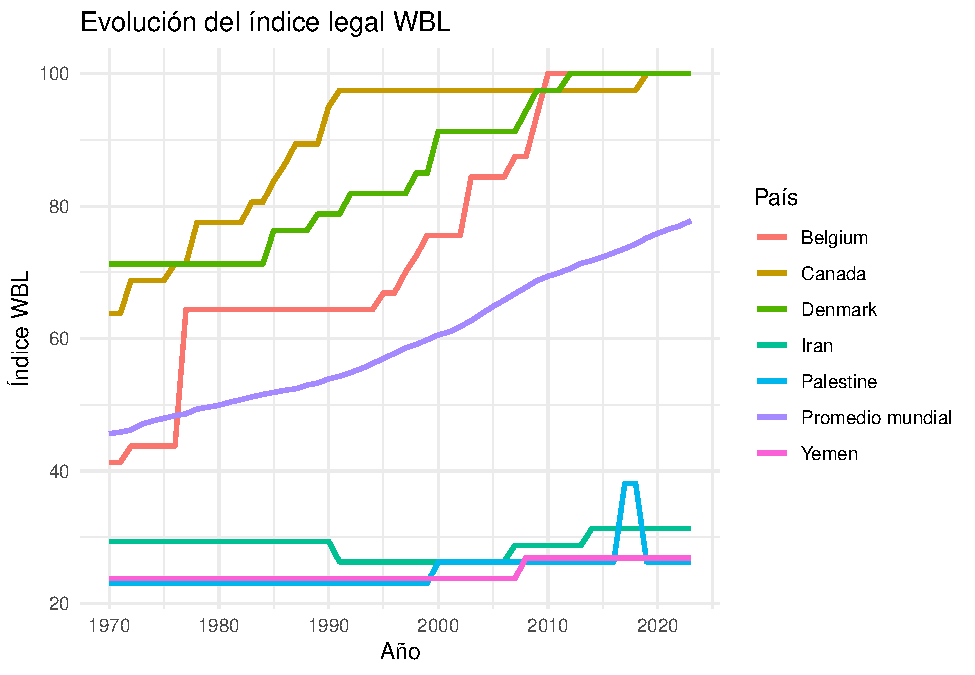
\includegraphics[width=\maxwidth]{figure/grafico-1} 

}

\caption[Evolución del índice WBL en países extremos y promedio mundial]{Evolución del índice WBL en países extremos y promedio mundial}\label{fig:grafico}
\end{figure}

\end{knitrout}

\subsection{Comentario}

El gráfico muestra cómo los países con mejores puntuaciones se mantienen cerca del valor máximo del índice (100 puntos), mientras que otros presentan trayectorias estancadas o con avances muy lentos.  
El promedio mundial crece de forma progresiva, aunque persisten importantes desigualdades estructurales.

\section{Conclusión}

El análisis del índice WBL permite visualizar con claridad las brechas legales de género en diferentes contextos geográficos.  
Este informe ha demostrado cómo, mediante un flujo reproducible con \texttt{knitr}, se pueden extraer conclusiones claras y respaldadas por datos reales.

\end{document}
